\section{Task 1}
\subsection{Problem Statement}
Implement and compare Insertion Sort, Counting Sort, and Merge Sort based on
various input size on randomly generated data.  The comparison metric should be
the execution time of each sorting algorithm.
\subsection{Code}
\begin{code}
    \caption{Code for generating random numbers and saving into a file nums.txt}
    \cppcode{../random_number.cpp}
    \label{code:random}
\end{code}

\begin{code}
    \caption{Code for insertion sort}
    \cppcode{../insertion_sort.cpp}
    \label{code:insertion}
\end{code}

\begin{code}
    \caption{Code for merge sort}
    \cppcode{../merge_sort.cpp}
    \label{code:merge}
\end{code}

\begin{code}
    \caption{Code for counting sort}
    \cppcode{../counting_sort.cpp}
    \label{code:counting}
\end{code}

\begin{code}
    \caption{Makefile}
    \inputminted[fontsize=\small]{make}{../Makefile}
\end{code}

\subsection{Output}
\begin{figure}[H]
    \centering
    \begin{subfigure}[b]{0.4\textwidth}
        \centering
        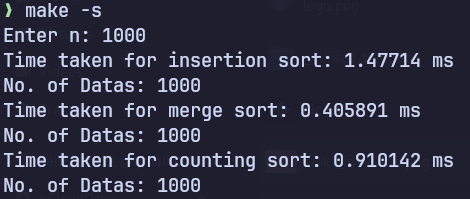
\includegraphics[width=\textwidth]{./img/out-1.png}
        \caption{Execution time for n=1000}
    \end{subfigure}
    \hfill
    \begin{subfigure}[b]{0.4\textwidth}
        \centering
        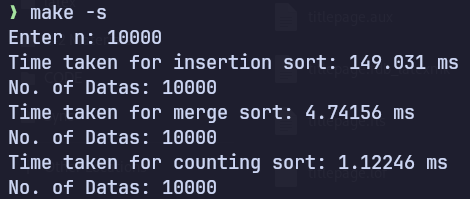
\includegraphics[width=\textwidth]{./img/out-2.png}
        \caption{Execution time for n=10000}
    \end{subfigure}
    \hfill
    \begin{subfigure}[b]{0.4\textwidth}
        \centering
        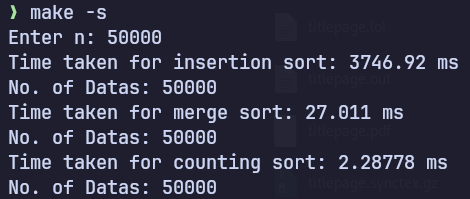
\includegraphics[width=\textwidth]{./img/out-3.png}
        \caption{Execution time for n=50000}
    \end{subfigure}
    \hfill
    \begin{subfigure}[b]{0.4\textwidth}
        \centering
        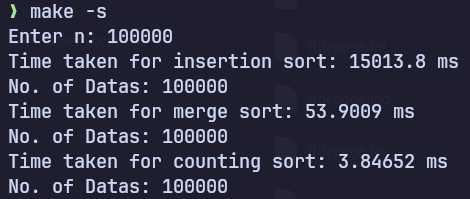
\includegraphics[width=\textwidth]{./img/out-4.png}
        \caption{Execution time for n=100000}
    \end{subfigure}
    
    \caption{Output for soting algorithm execution time}

\end{figure}

\subsection{Result Analysis \& Discussion}
\begin{figure}[H]
    \centering
    \begin{subfigure}[b]{0.4\textwidth}
        \centering
        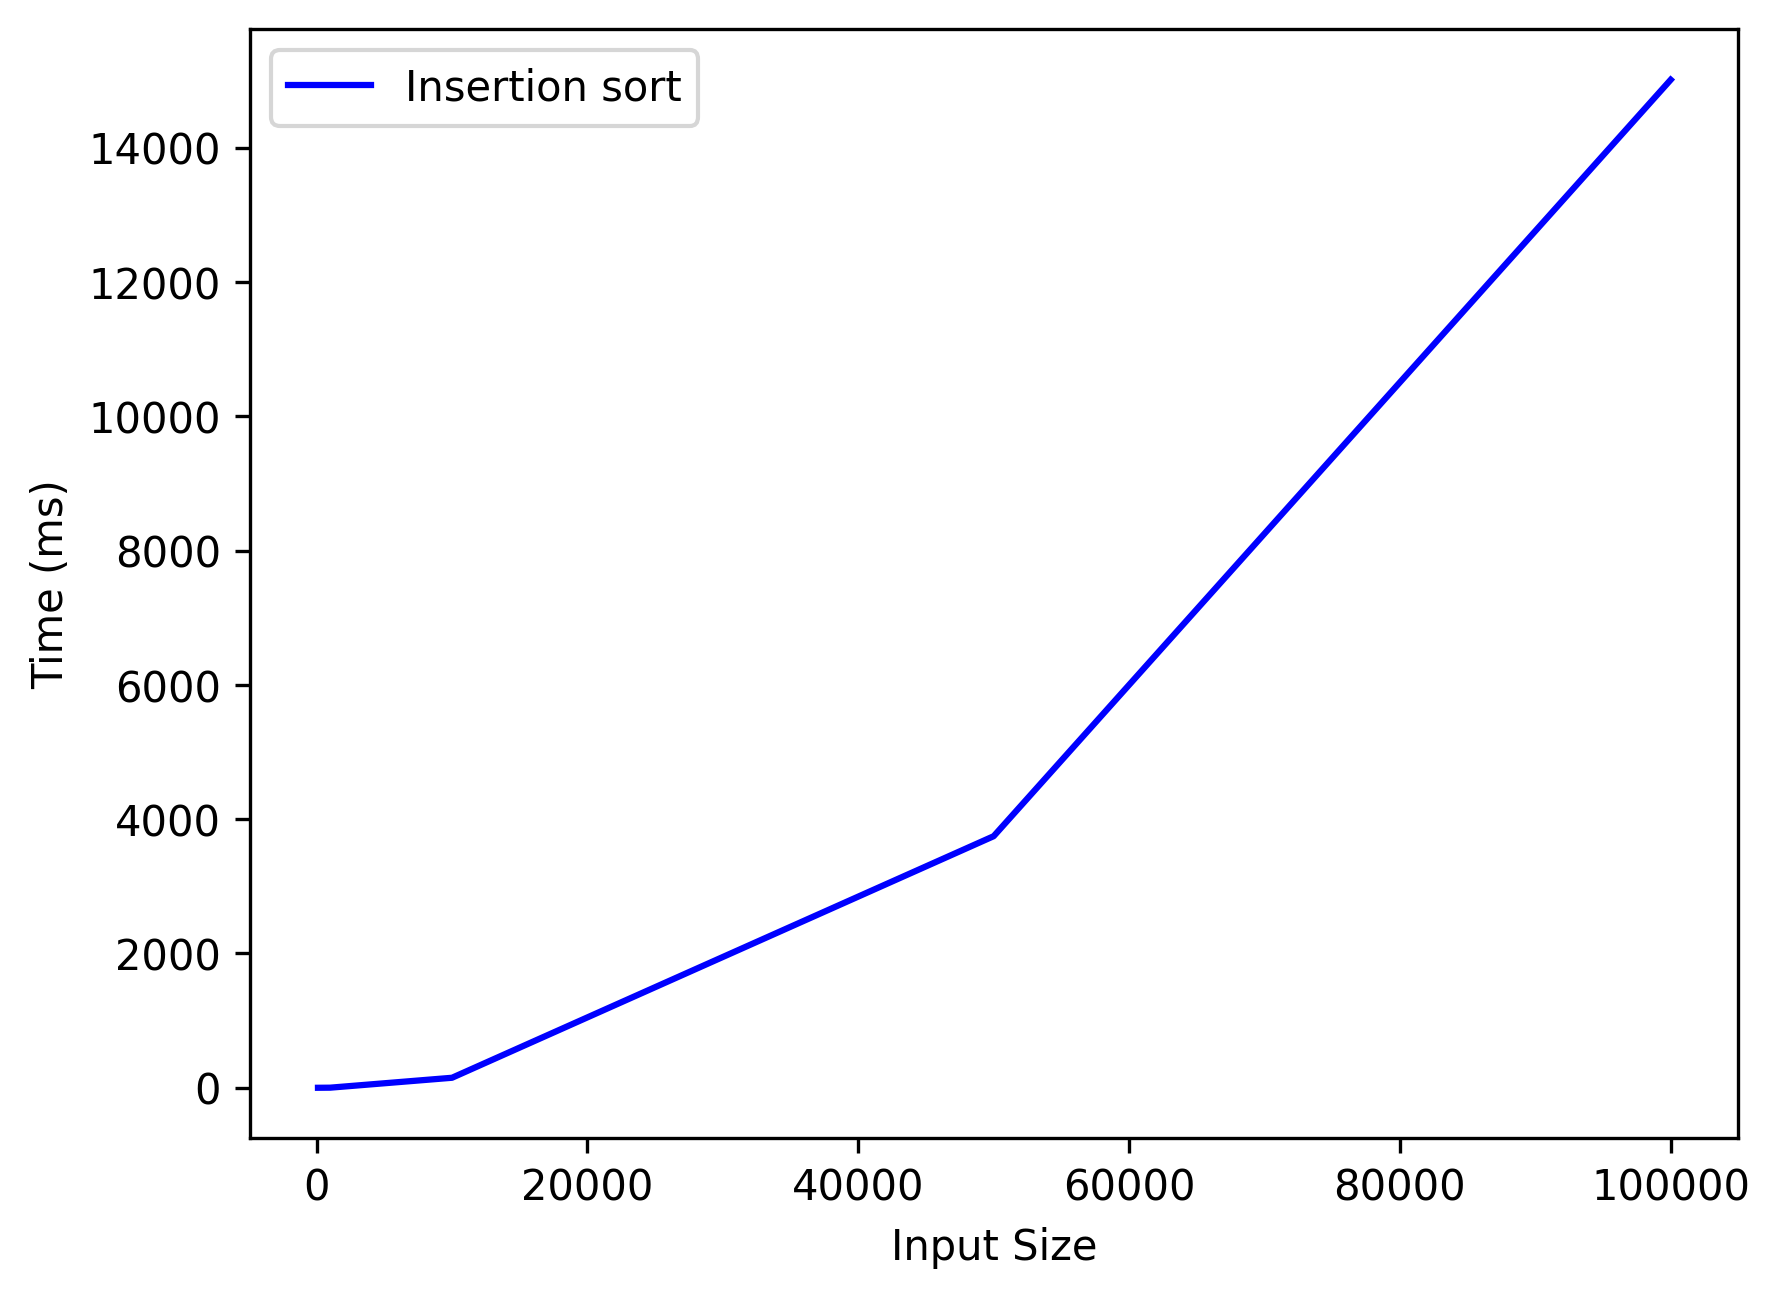
\includegraphics[width=\textwidth]{task1_insertion.png}
    \end{subfigure}
    \hfill
    \begin{subfigure}[b]{0.4\textwidth}
        \centering
        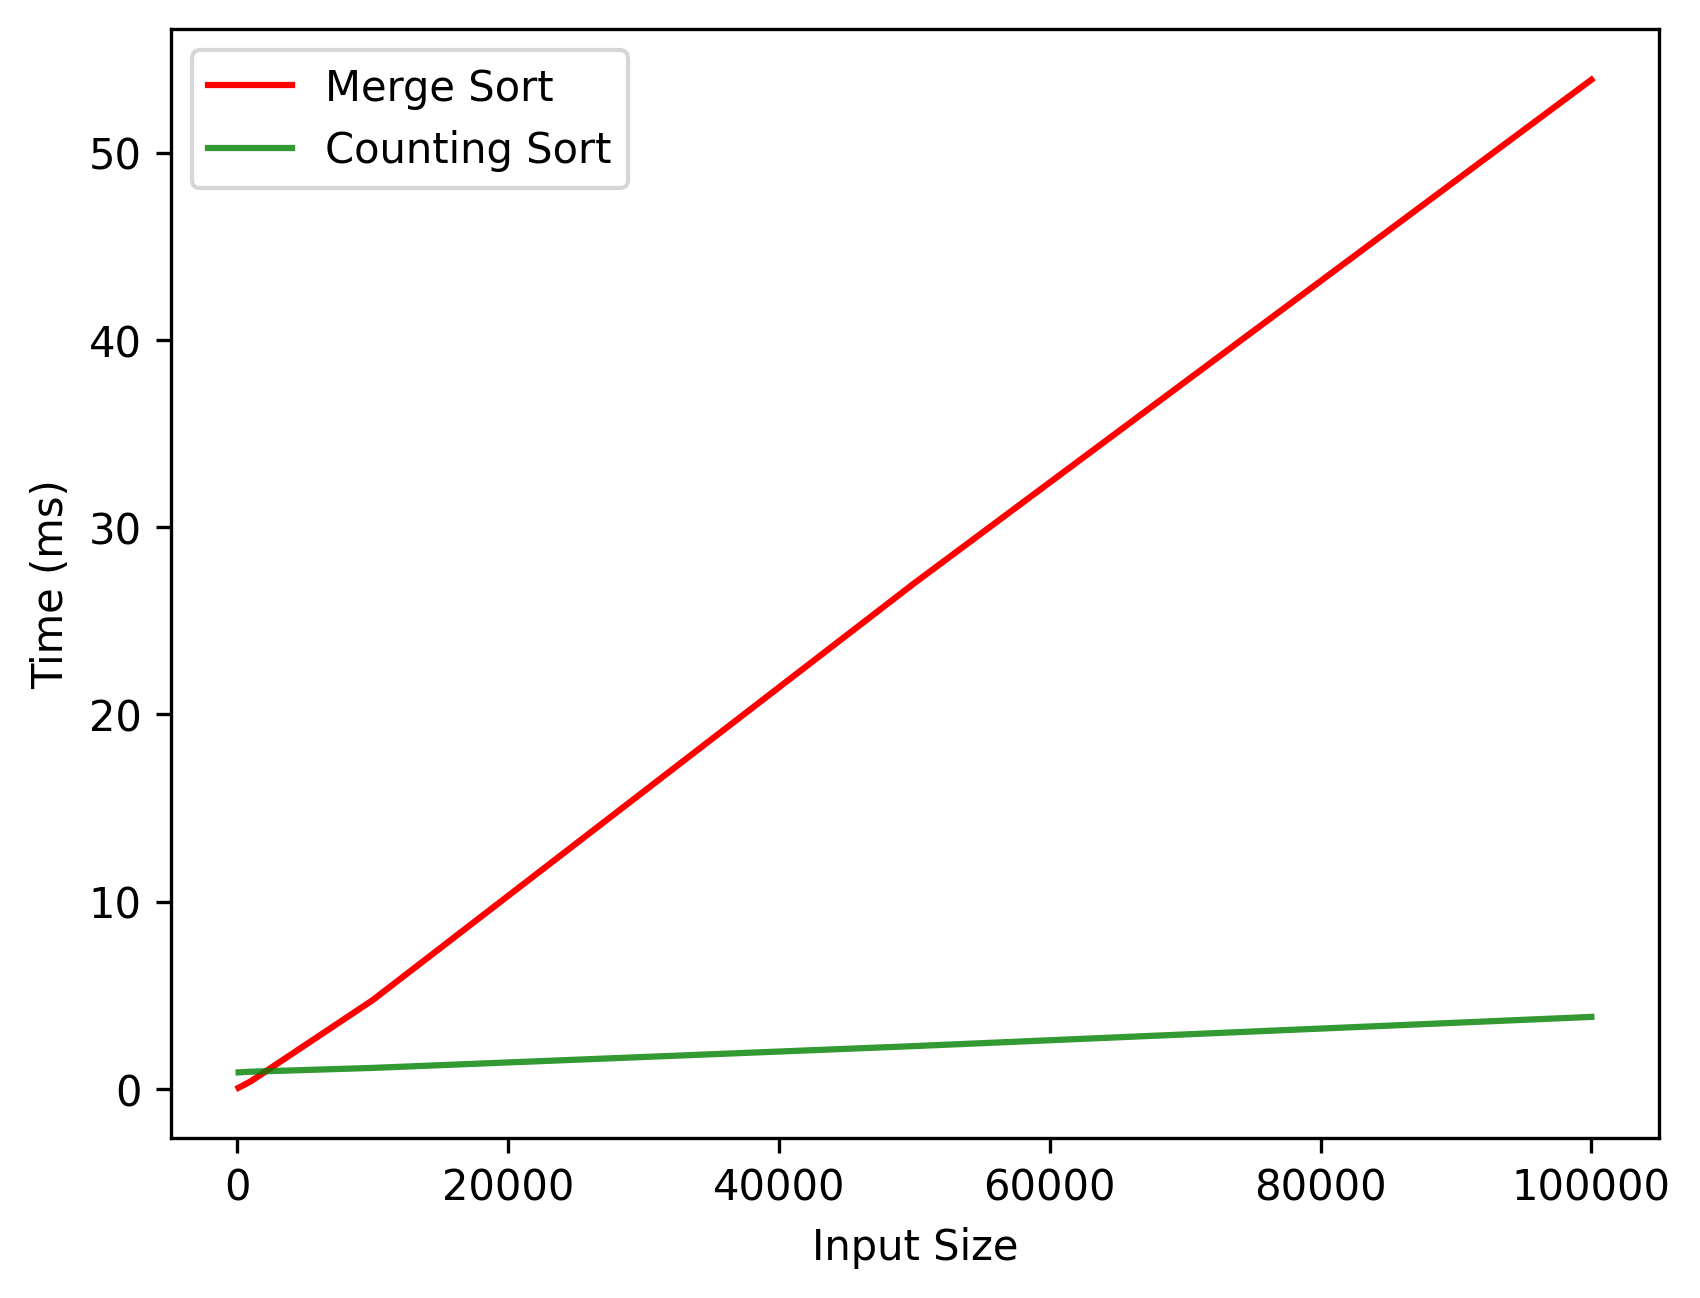
\includegraphics[width=\textwidth]{task1_merge_count.png}
    \end{subfigure}

    \caption{Time vs. Input size plot for insertion, merge and counting sort}
\end{figure}

\newpage
\section{Task 2}
\subsection{Problem Statement}
Implement a Hybrid Sort algorithm where the algorithm switches from Merge Sort
to Insertion Sort when the size of the subarray to be conquered becomes smaller
than a threshold. Determine the optimal threshold empirically. Compare this
Hybrid Sort algorithm with Merge Sort  based on various input size and various
threshold on randomly generated data.
\subsection{Code}
\begin{code}
    \label{code:hybrid}
    \caption{Code for hybrid sort}
    \cppcode{../hybrid_sort.cpp}
\end{code}
\subsection{Output}
\subsection{Result Analysis \& Discussion}

\newpage
\section{Task 3}
\subsection{Problem Statement}
Take the Hybrid Sort algorithm from Task 2, instead of Insertion Sort, use
Bubble Sort. Determine the optimal threshold empirically. Make a 3-way
comparison between Merge Sort, Hybrid Sort with Insertion Sort, Hybrid Sort
with Bubble Sort algorithm based on various input size and various threshold on
randomly generated data.
\subsection{Code}
\begin{code}
    \label{code:bubble}
    \caption{Code for hybrid sort with bubble sort}
    \cppcode{../bubble.cpp}
\end{code}
\subsection{Output}
\begin{figure}[H]
    \centering
    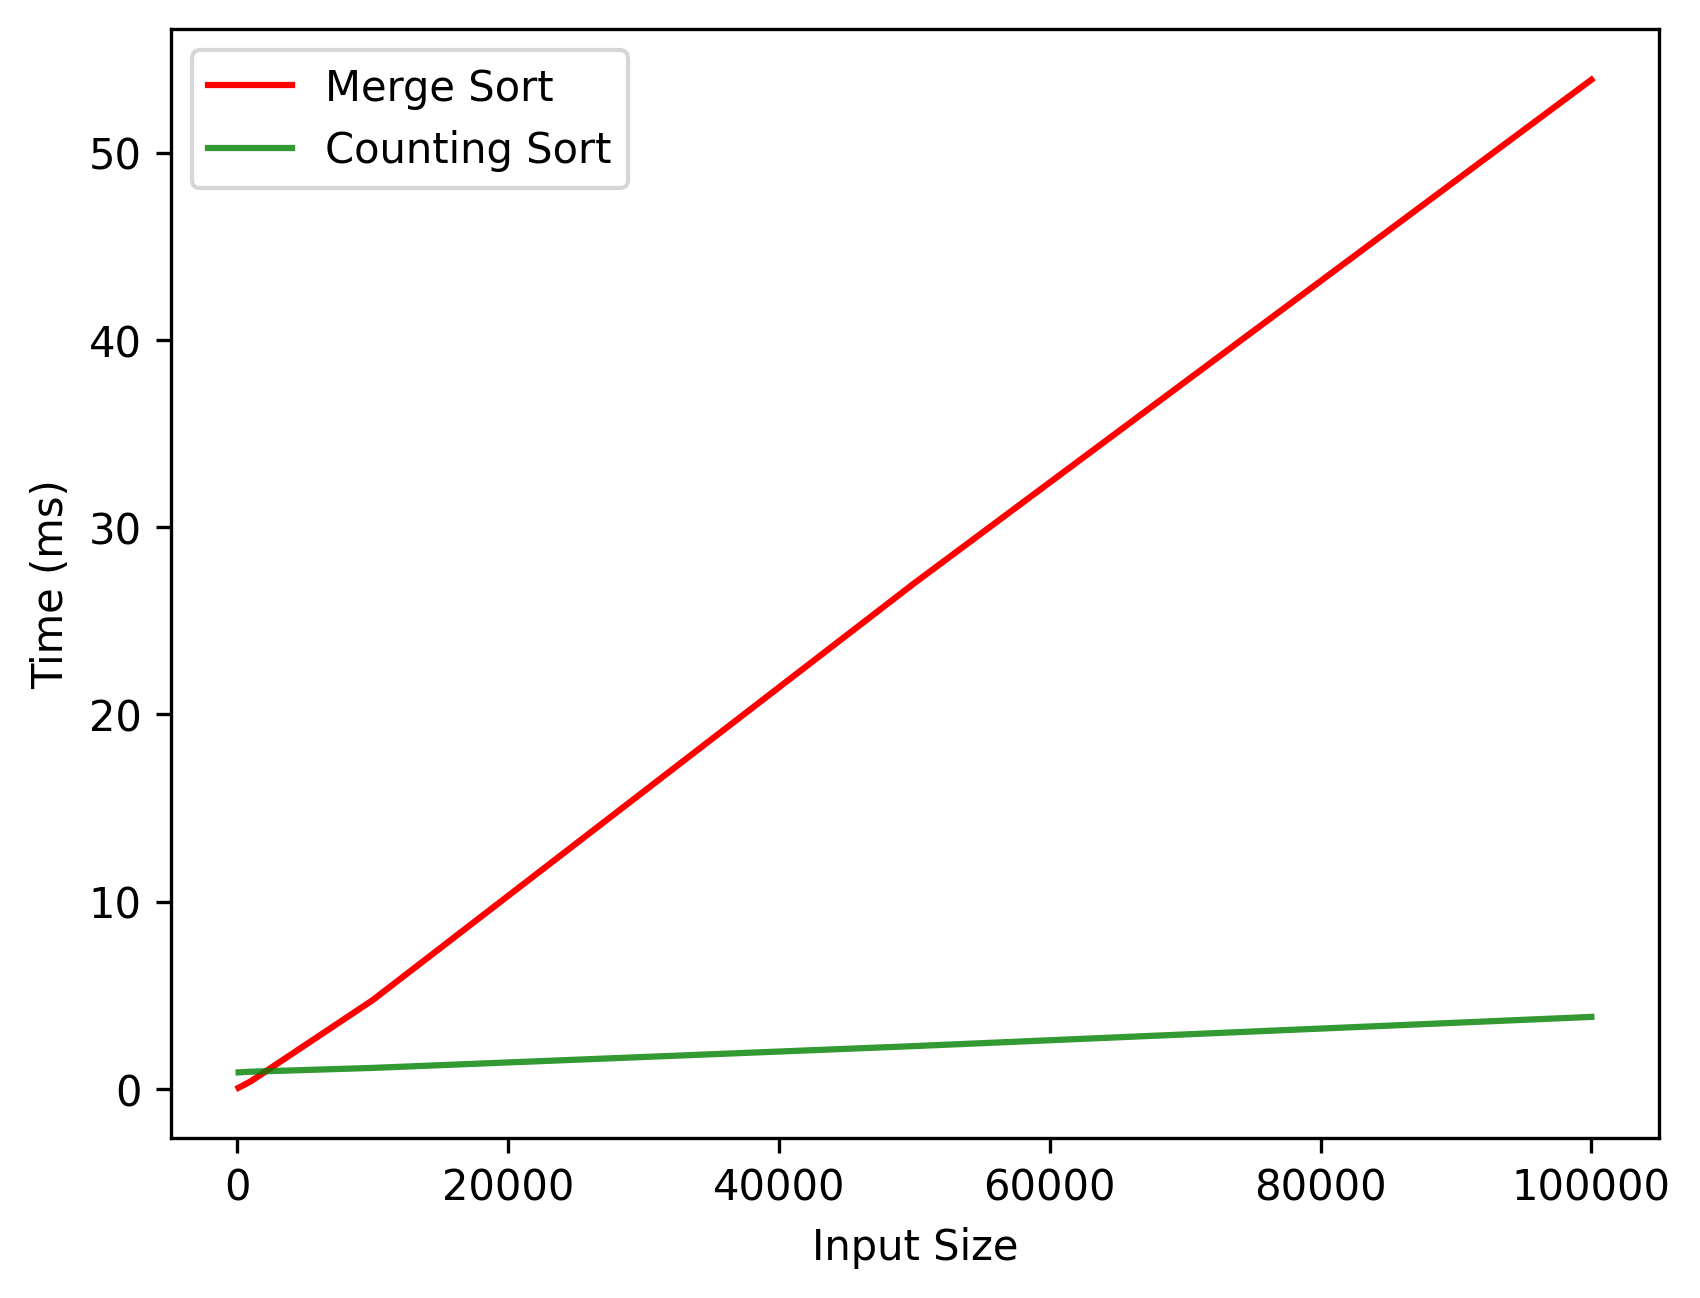
\includegraphics[width=0.7\textwidth]{task1_merge_count.png}
\end{figure}
\subsection{Result Analysis \& Discussion}

\begin{table}[H]
    \centering
    \caption{3-way comparison table for merge \& hybrid sort}
    \label{tab:comp}
\begin{tabular}{llrr}
    \toprule
    \multicolumn{4}{c}{Sorting Algorithm} \\
    \cmidrule(r){2-4}
    Property & Merge Sort & Hybrid w/ insertion sort & Hybrid w/ bubble sort \\
    \midrule
    Gnat & per gram & 13.65 \\
    & each & 0.01 \\
    Gnu & stuffed & 92.50 \\
    Emu & stuffed & 33.33 \\
    Armadillo & frozen & 8.99 \\
    \bottomrule
\end{tabular}
\end{table}

\section{Task 4}
\subsection{Problem Statement}

\subsection{Code}
\begin{code}
    
\end{code}

\subsection{Output}
